\section{}
\[
H(s)=\frac{10}{s+10}\,.
\]
\subsection{Bode-Diagramm}
\begin{center}
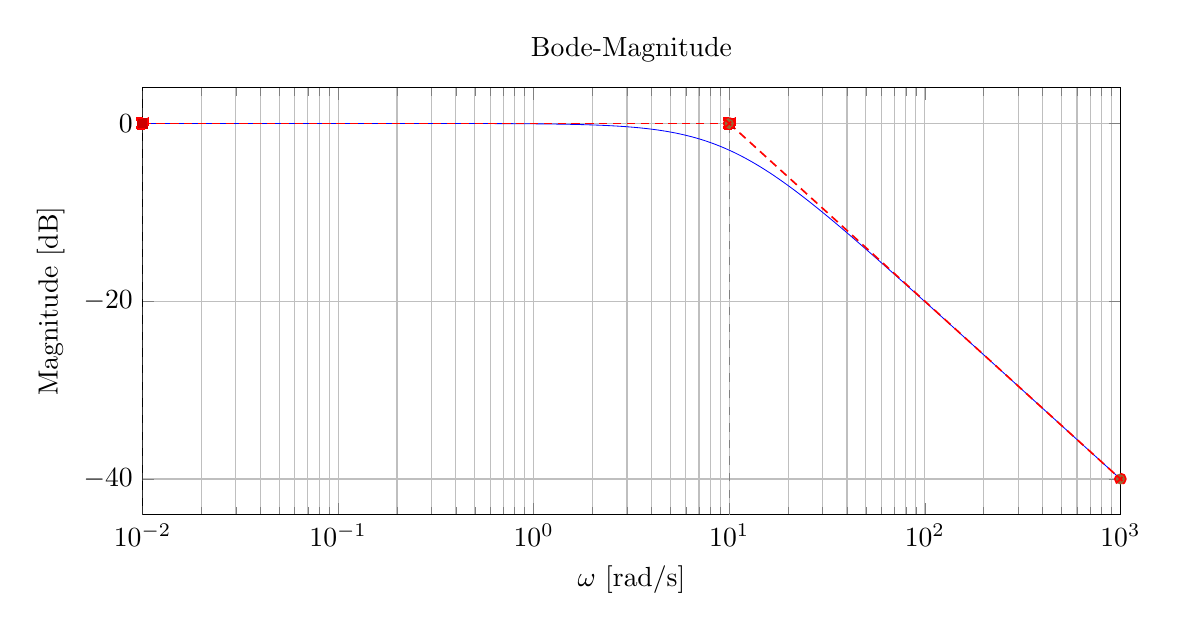
\begin{tikzpicture}
\begin{semilogxaxis}[
  width=14cm,height=7cm,
  xmin=1e-2,xmax=1e3,
  xlabel={$\omega$ [rad/s]},
  ylabel={Magnitude [dB]},
  grid=both,
  ytick distance=20, 
  title={Bode-Magnitude}
]
\addplot[
  domain=1e-2:1e3,
  samples=600,
  mark=none,
  line width=0.3pt,
  blue
] {-20*ln(sqrt(1 + (x/10)^2))/ln(10)};
\addplot+[domain=1e-2:1e1,samples=2,dashed,dash pattern=on 3pt off 2pt,line width=0.6pt,red] {0};
\addplot+[domain=1e1:1e3,samples=2,dashed,dash pattern=on 3pt off 2pt,line width=0.6pt,red] {-20*ln(x/10)/ln(10)};
\draw[gray,dashed] (rel axis cs:0,0) -- (rel axis cs:0,1);
\draw[gray,dashed] (axis cs:10,\pgfkeysvalueof{/pgfplots/ymin}) -- (axis cs:10,\pgfkeysvalueof{/pgfplots/ymax});
\node[gray,anchor=south east] at (axis cs:10,\pgfkeysvalueof{/pgfplots/ymax}) {\scriptsize Pol $\omega_p=10$};
\end{semilogxaxis}
\end{tikzpicture}
\vspace{6mm}
\begin{tikzpicture}
\begin{semilogxaxis}[
  width=14cm,height=7cm,
  xmin=1e-2,xmax=1e3,
  ytick distance 45,
  ymin=-95,ymax=5,
  xlabel={$\omega$ [rad/s]},
  ylabel={Phase [°]},
  grid=both,
  title={Bode-Phase}
]
\addplot[
  domain=1e-2:1e3,
  samples=600,
  mark=none,
  line width=0.3pt,
  blue
] {-atan(x/10)};
\addplot+[domain=1e-2:1e0,samples=2,dashed,dash pattern=on 3pt off 2pt,line width=0.6pt,red] {0};
\addplot+[domain=1e0:1e2,samples=2,dashed,dash pattern=on 3pt off 2pt,line width=0.6pt,red] {-45 - 45*ln(x/10)/ln(10)};
\addplot+[domain=1e2:1e3,samples=2,dashed,dash pattern=on 3pt off 2pt,line width=0.6pt,red] {-90};
\draw[gray,dashed] (rel axis cs:0,0) -- (rel axis cs:0,1);
\draw[gray,dashed] (axis cs:10,\pgfkeysvalueof{/pgfplots/ymin}) -- (axis cs:10,\pgfkeysvalueof{/pgfplots/ymax});
\node[gray,anchor=south east] at (axis cs:10,\pgfkeysvalueof{/pgfplots/ymax}) {\scriptsize Pol $\omega_p=10$};
\end{semilogxaxis}
\end{tikzpicture}
\end{center}
\newpage
\subsection{Erklärung}
\vspace{5mm}
\begin{description}[leftmargin=1.2em,labelsep=.6em,font=\bfseries]
\item[Schritt 1] DC-Faktor $1$: $H(s)=\frac{10}{s+10}=\frac{1}{1+s/10}$, daher für $\omega\ll10$ gilt $|H(\j\omega)|\approx1$; Betrag liegt bei $0\,\mathrm{dB}$ ohne Anfangssteigung, Phase $\approx0^\circ$.
\item[Schritt 2] Einfacher Pol bei $\omega_p=10\,\mathrm{rad/s}$: ab $\omega=10$ wechselt die Magnituden-Steigung um $-20\,\mathrm{dB/dec}$; die exakte Dämpfung am Eckpunkt beträgt $-10\log_{10}2\approx-3.01\,\mathrm{dB}$. Die Phasenübergangsdekade liegt zwischen $\omega_l=1$ und $\omega_h=100\,\mathrm{rad/s}$.
\item[Schritt 3] Grenzverhalten: für $\omega\gg10$ folgt $|H(\j\omega)|_{\mathrm{dB}}\approx-20\log_{10}(\omega/10)$; die Phase fällt in der Übergangsdekade linearisiert von $0^\circ$ nach $-90^\circ$ (Näherung: $-45^\circ-45\log_{10}(\omega/10)$), mit $\angle H(\j\omega)=-45^\circ$ bei $\omega=10$.
\end{description}

\vspace{0.5cm}
\medskip
\noindent\textbf{Stückweise Näherung}
\[
|H(\j\omega)|_{\mathrm{dB}}\approx
\begin{cases}
0,& \omega\ll10,\\[4pt]
-10\log_{10}2,& \omega=10,\\[4pt]
-20\log_{10}(\omega/10),& \omega\gg10,
\end{cases}
\qquad
\]
\newpage